% !TEX root = ../geometry.tex

\chapter{Polygons}

%--------------------------------------------------------------------------------------------
			\section{Terminology}
%--------------------------------------------------------------------------------------------

The definition of a polygon is fairly technical, 
and it is not important that you know it word for word.

The important characteristics of a polygon are that it is a shape
created with some number of segments that is \emph{closed}. 
Polygons cannot have rounded sides, and they cannot cross themselves.

	\begin{center}
	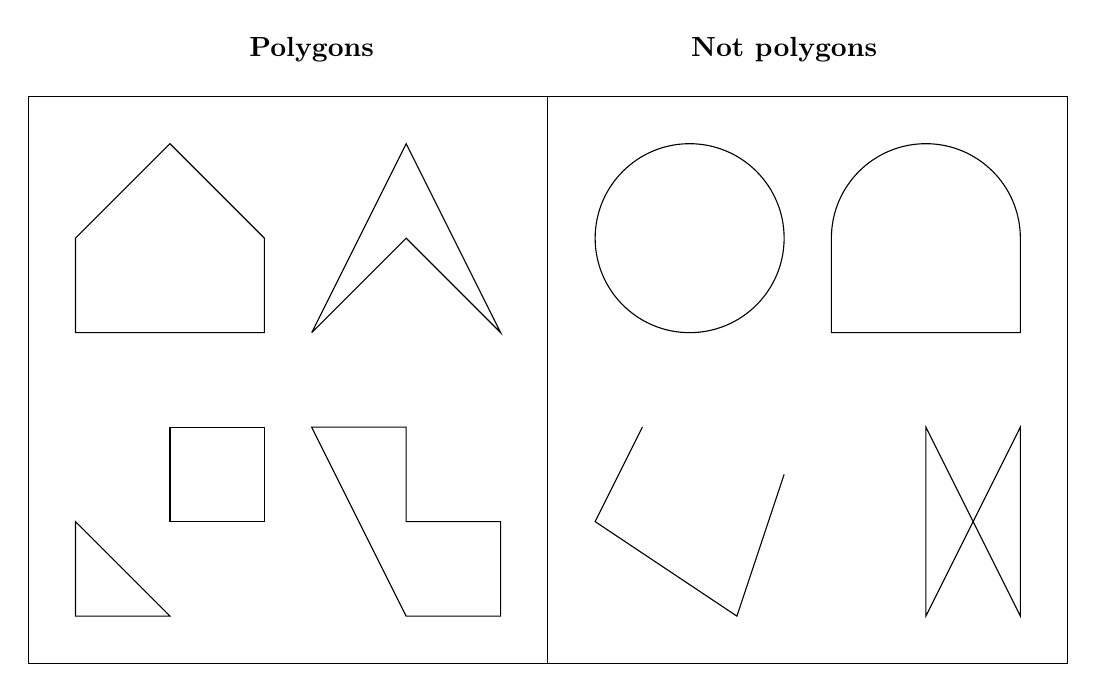
\begin{tikzpicture} [scale=1.2]
		\node at (-2.5,0) {\bfseries Polygons};
		\draw (-5,-2) -- ++(0,-1) -- ++ (2,0) -- ++ (0,1) -- ++ (-1,1) -- ++ (-1,-1);
		\draw (-2.5,-3) -- ++ (1,2) -- ++ (1,-2) -- ++ (-1,1) -- ++ (-1,-1);
		\draw (-4,-5) rectangle (-3,-4);
		\draw (-2.5,-4) -- ++ (1,0) -- ++ (0,-1) -- ++ (1,0) -- ++ (0,-1) -- ++(-1,0)-- cycle;
		\draw (-5,-6) -- (-4,-6) -- (-5,-5) -- cycle;
		
		\node at (2.5,0) {\bfseries Not polygons};
		\draw (1.5,-2) circle (1);
		\draw (3,-2) -- ++ (0,-1) -- ++ (2,0) -- ++ (0,1) arc (0:180:1);
		\draw (1,-4) -- (.5,-5) -- (2,-6) -- (2.5,-4.5);
		\draw (4,-4) -- (4,-6) -- (5,-4) -- (5,-6) -- cycle;
		
		\draw (-5.5, -6.5) rectangle (0,-.5);
		\draw (5.5, -6.5) rectangle (0,-.5);
	\end{tikzpicture}
	\end{center}
	
\newpage	

\subsection{Naming polygons}

Polygons are given more specific names based on how many sides they have.
You already know (at least) two of these names. 
\emph{Triangles} and \emph{quadrilaterals} are both polygons,
with three and four sides, respectively.

You need to know the common names given in 
%Table~\ref{table:polygon-names}\footnote{
Table 11.1\footnote{
The name for an 11-sided polygon is undecagon,
but nobody uses that word---not even at math parties---so 
you don't need to know it.}:
%\begin{table}
%\centering
%\caption{Common names of polygons by number of sides}
\begin{center}
Table 11.1:  Common names of polygons by number of sides\\

\label{table:polygon-names}
\begin{tabular}{@{ } c l  c  c l @{ }}
\toprule
{\bfseries Sides}&{\bfseries Name} &  \qquad \qquad & {\bfseries Sides}&{\bfseries Name} \\
\cmidrule(lr){1-2}\cmidrule(lr){4-5}
3 & triangle 	&& 8 		& octagon \\
4 & quadrilateral && 9		& nonagon\\
5 & pentagon 	&& 10 		& decagon\\
6 & hexagon 	&& 12 		& dodecagon\\
7 & heptagon 	&& $n$	& n-gon \\
\bottomrule
\end{tabular}
\end{center}

\vspace{0.5cm}

%\end{table}
What if a polygon doesn't have a specific name? 
What do you call a polygon with 21 sides?
The answer is that you can name any polygon a ``number-of-sides-gon''.
A 21-sided polygon is called a \emph{21-gon}. 
A 98-sided polygon is called a \emph{98-gon}.
A polygon with $n$ sides is called an $n$-gon.
But, if there is a common name, use that first.
Everybody will look at you funny if you call a triangle a 3-gon,
even though it is.\\

As a final point, 
notice that the number of sides is always the same as the number of angles,
and that is always the same as the number of vertices.
An octagon, for example, has 8 sides, 8 angles, and 8 vertices.

\subsection{Diagonal}

In Section \ref{sec:quad-intro}, 
you drew diagonals in quadrilaterals. 
The definition of a diagonal can be extended to apply to any polygon.

A \textbf{diagonal} is a segment connecting two non-consecutive vertices of a polygon.
You can usually draw many diagonals from each vertex,
and as usual, they can all be different lengths.

\newpage

Below is a hexagon in which all possible diagonals are drawn from one vertex.
	\begin{center}
	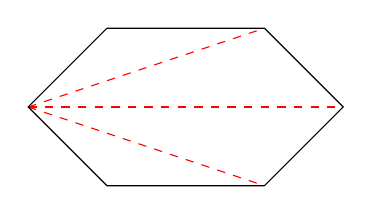
\begin{tikzpicture}
		\begin{scope}[red,dashed]
			\draw (-2,0) -- (1,1);
			\draw (-2,0) -- (2,0);
			\draw (-2,0) -- (1,-1);
		\end{scope}
		\draw (-2,0) -- (-1,1) -- (1,1) -- (2, 0) -- (1,-1) -- (-1,-1) -- cycle;
	\end{tikzpicture}
	\end{center}
\noindent \q If a hexagon has six vertices, why are there only \emph{three} possible diagonals from a vertex?

\medskip

\noindent \q If you can draw three diagonals from a vertex, 
how many diagonals will there be in the entire hexagon?

\medskip

\noindent \q By counting carefully, 
determine the total number of diagonals in the hexagon below,
in which every diagonal is drawn.
Does it match your prediction?
If not, double-check the count, or improve your prediction!
	\begin{center}
	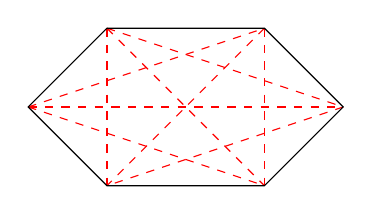
\begin{tikzpicture}
		\begin{scope}[red,dashed]
			\draw (-2,0) -- (1,1);
			\draw (-2,0) -- (2,0);
			\draw (-2,0) -- (1,-1);
			\draw (-1,1) -- (2,0);
			\draw (-1,1) -- (1,-1);
			\draw (-1,1) -- (-1,-1);
			\draw (1,1) -- (1,-1);
			\draw (1,1) -- (-1,-1);
			\draw (2,0) -- (-1,-1);
		\end{scope}
		\draw (-2,0) -- (-1,1) -- (1,1) -- (2, 0) -- (1,-1) -- (-1,-1) -- cycle;
	\end{tikzpicture}
	\end{center}

\noindent \q Is the total number of diagonals in a hexagon a constant,
or can it change? 
To help you answer\footnote{
What kind of reasoning are you using?}, a different hexagon is sketched below. 
See if it has the same number of diagonals.
	\begin{center}
	\begin{tikzpicture}
		\draw (-3,2) -- (0,1.5) -- (3,2) -- (3,-2) -- (0,-1.5) -- (-3,-2) -- cycle;
	\end{tikzpicture}
	\end{center}


\subsection{Convex and concave}

As you were drawing the diagonals in the last example,
you may have noticed that they were not all inside the hexagon.

When one or more diagonals lie outside the polygon,
the polygon is called \textbf{concave}.
A \textbf{convex} polygon is one in which all the diagonals lie inside the polygon.

Most people get pretty good at identifying convex and concave polygons by sight.
\q Can you label the pictures below with a polygon name and whether it is convex or concave?
	\begin{center}
	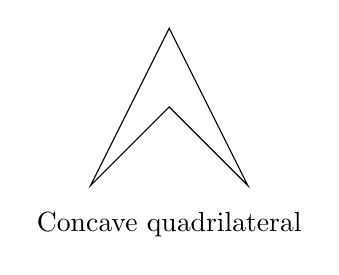
\begin{tikzpicture}
		\draw (-1,0) -- (0,2) -- (1,0) -- (0,1) -- cycle;
		\node at (0,-.5) {Concave quadrilateral};
	\end{tikzpicture}
	\hspace{1cm}
	\begin{tikzpicture}
		\draw (90:1) -- (162:1) -- (234:1) -- (306:1) -- (18:1) -- cycle;
		\node at (0,-1.5) {\proofblank};
	\end{tikzpicture}
	\hspace{1cm}
	\begin{tikzpicture}
		\draw (22.5:.5) -- (67.5:1) -- (112.5:1) -- (157.5:1)
			-- (202.5:1) -- (247.5:1) -- (292.5:1) -- (337.5:1) -- cycle;
		\node at (0,-1.5) {\proofblank};
	\end{tikzpicture}
	\end{center}

\subsection{Regular}

A polygon is called \textbf{equilateral} if all its sides are congruent.
A polygon is called \textbf{equiangular} if all its angles are congruent.

In a triangle, being equilateral and being equiangular are the same thing,
but in every other polygon, they are different. 
For example,
a rectangle is an example of a quadrilateral 
that is equiangular but not necessarily equilateral.
A rhombus, of course,
is an example of a quadrilateral that is equilateral but not
necessarily equiangular.
If you are ever tempted to think that equilateral and equiangular are the same thing,
remember the rectangle and the rhombus! \q Sketch and mark one of each and label them as equilateral and equiangular.

\bigskip

Of course, it is completely possible for a polygon to be both equilateral and equiangular.
Such polygons are called \textbf{regular}. 
For most polygons, you just say ``regular pentagon'' or ``regular octagon'', etc.,
but a ``regular quadrilateral'' has a special name. \q What is it?

\medskip
\newpage

\noindent \q Consider the three pentagons below.  For each, write the best word: equilateral, equiangular, or regular.\\\\

	\hspace*{\fill}
	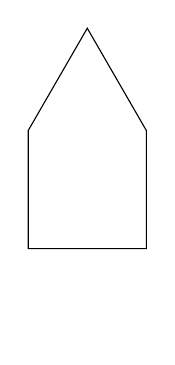
\begin{tikzpicture}
		\draw (-.75,0) -- (-.75,1.5) -- (0,{1.5+.75*sqrt(3)}) -- (.75,1.5) -- (.75,0) -- cycle;
		\node at (0,-1) {\proofblank};	
	\end{tikzpicture}
	\hspace*{\fill}
	\begin{tikzpicture}
		\draw (90:1.5) -- (162:1.5) -- (234:1.5) -- (306:1.5) -- (18:1.5) -- cycle;
		\node at (0,-2.5) {\proofblank};
	\end{tikzpicture}
	\hspace*{\fill}
	\begin{tikzpicture}
		\draw (0,0) coordinate (a) -- (1.25,0) coordinate (b);
		\draw (b) -- ($(b)!1.5cm!108:(a)$) coordinate (c);
		\draw (c) -- ($(c)!1.75cm!108:(b)$) coordinate (d);
		\path [name path = froma] (a) -- ($(a) ! 2cm ! -108:(b) $);
		\path [name path = fromd] (d) -- ($(d) ! 1.5cm ! 108:(c)$);
		\path [name intersections={of = froma and fromd, by = e}];
		\draw (a) -- (e) -- (d);
		\node at (0.5,-3.5) {\proofblank};
	\end{tikzpicture}
	\hspace*{\fill}

\noindent Regular polygons will play an important role in this chapter.  


\subsection{Circumscribed and inscribed}

You will recall that all triangles could be circumscribed by a circle.  Hopefully, it is also clear that we found the \emph{circumcenter}\footnote{center of the circumcircle} by finding the intersection point of the perpendicular bisectors of the three sides of the triangle.  All three perpendicular bisectors always intersect at one point.\\

We recently examined what had to be the case if a quadrilateral could be inscribed in a circle.\footnote{The opposite angles must be supplementary.} It was implied that if a quadrilateral had opposite supplementary angles then a circle could also be circumscribed about the quadrilateral.  It also follows the pattern that a circumcenter of a quadrilateral can be found at the intersection of all of the perpendicular bisectors.  All four perpendicular bisectors do not always intersect at the same point. \q Can you name a special quadrilateral or two for which all of the perpendicular bisectors do not intersect at one point?

\medskip

\noindent \q Sketch the perpendicular bisectors of each side of the pentagons above.  Do they all intersect at the same point for each pentagon?  What does this mean for pentagons and other polygons with more sides.

\medskip
\newpage

As you may have guessed, it is a fact that all regular polygons can be circumscribed by a circle and consequently can be inscribed in a circle.  While regular polygons are not the only polygons that can be circumscribed by a circle, we will focus on regular polygons in this book.  You will see that polygons---especially regular polygons---appear in problems with other shapes, notably circles.  You will recall:  
the terms \emph{circumscribed} (i.e., drawn around) 
and \emph{inscribed} (i.e., drawn inside) appear frequently to describe these figures.

To describe the figure on the left, you could say 
\textit{a circle circumscribed about a triangle} or 
\textit{a triangle inscribed in a circle}.\\

\hspace*{\fill}
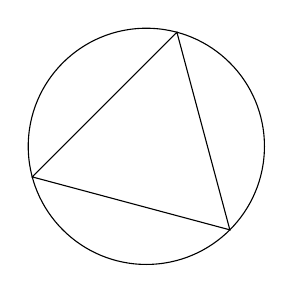
\begin{tikzpicture}
	\draw (0,0) coordinate (o) circle (1.5);
	\draw (75:1.5) -- (195:1.5) -- (315:1.5) -- cycle;
	\fillpoints {o}
\end{tikzpicture}
\hspace*{\fill}
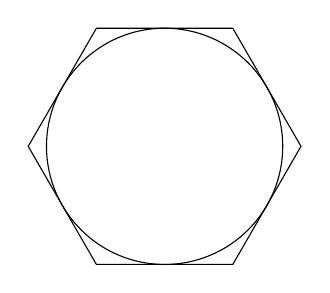
\begin{tikzpicture}
	\draw (0,0) coordinate (o) circle (1.5);
	\draw (0:1.732) -- (60:1.732) -- (120:1.732) -- (180:1.732) -- (240:1.732) -- (300:1.732) -- cycle;
	\fillpoints {o}
\end{tikzpicture}
\hspace*{\fill}

\noindent \q Describe the figure on the right in two ways.

\medskip

\noindent **To clarify the definitions, a polygon is inscribed in a circle
if and only if each of its vertices is on the circle.
A polygon is circumscribed about a circle,
if and only if each of its sides is \emph{tangent} to the circle.

\begin{exercises}

	\begin{ex} \e Make note cards for:  \textbf{Polygon}, \textbf{Polygon Names}, \textbf{Diagonal}, \textbf{Convex/Concave}, \textbf{Regular}, \textbf{Circumscribed/Inscribed}
	\begin{sol}
	Note cards
	\end{sol}
	\end{ex}
	
	\begin{ex}
	\e Sketch the following:
	
	(a) a concave hexagon \hspace*{\fill} (b) A regular octagon
	
	\begin{sol}
	
	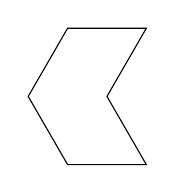
\begin{tikzpicture} 
		\draw (0,0) -- (60:1) -- (120:1) -- (180:1) -- (240:1) -- (300:1) -- cycle;
	\end{tikzpicture}
	,
	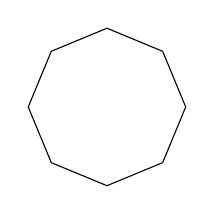
\begin{tikzpicture} 
		\draw (0:1) -- (45:1) -- (90:1) -- (135:1)
			-- (180:1) -- (225:1) -- (270:1) -- (315:1) -- cycle;
	\end{tikzpicture}
	\end{sol}
	\end{ex}
	
	\medskip
	\newpage

	\begin{ex} \e Construct (or sketch accurately) the circumcenters for the following regular polygons.  If you have a compass, use it to circumscribe a circle about the polygons.\\\\

\begin{center}
\begin{tikzpicture} %[scale=0.8]
			\coordinate (A) at (0,0);
			\coordinate (B) at (3,0);
			\coordinate (C) at ($(B)!3cm!-108:(A)$);
			\coordinate (D) at ($(C)!3cm!-108:(B)$);
			\coordinate (E) at ($(D)!3cm!-108:(C)$);
			\draw (A)--(B) node [below, midway] {} --(C)--(D)  --(E)--(A) ;
			
			\coordinate (A) at (7,0);
			\coordinate (B) at (9.5,0);
			\coordinate (C) at ($(B)!2.5cm!-120:(A)$);
			\coordinate (D) at ($(C)!2.5cm!-120:(B)$);
			\coordinate (E) at ($(D)!2.5cm!-120:(C)$);
			\coordinate (F) at ($(E)!2.5cm!-120:(D)$);
			\draw (A)--(B) --(C)--(D) --(E)-- (F) --(A) ;
			
			\coordinate (A) at (0,-7.5);
			\coordinate (B) at (2,-7.5);
			\coordinate (C) at ($(B)!2cm!-135:(A)$);
			\coordinate (D) at ($(C)!2cm!-135:(B)$);
			\coordinate (E) at ($(D)!2cm!-135:(C)$);
			\coordinate (F) at ($(E)!2cm!-135:(D)$);
			\coordinate (G) at ($(F)!2cm!-135:(E)$);
			\coordinate (H) at ($(G)!2cm!-135:(F)$);
			\draw (A)--(B) --(C)--(D) --(E) -- (F) -- (G) --(H)--(A) ;
			
			\coordinate (A) at (7,-7.5);
			\coordinate (B) at (8.75,-7.5);
			\coordinate (C) at ($(B)!1.75cm!-140:(A)$);
			\coordinate (D) at ($(C)!1.75cm!-140:(B)$);
			\coordinate (E) at ($(D)!1.75cm!-140:(C)$);
			\coordinate (F) at ($(E)!1.75cm!-140:(D)$);
			\coordinate (G) at ($(F)!1.75cm!-140:(E)$);
			\coordinate (H) at ($(G)!1.75cm!-140:(F)$);
			\coordinate (I) at ($(H)!1.75cm!-140:(G)$);
			\draw (A)--(B) --(C)--(D) --(E) -- (F) -- (G) --(H)--(I)--(A) ;
\end{tikzpicture}
\end{center}

	\begin{sol}
	Constructions/Sketches
	\end{sol}
	\end{ex}
	
	\begin{ex} \e In the regular polygons above, which ones have diagonals that could also be described as diameters of their circumcircles?  Is there a pattern to this relationship?
	\begin{sol}
	The hexagon and octagon do and the pentagon does not.  If a regular polygon has an even number of sides, then it has diagonals that share space with its circumcircle's diameters.
	\end{sol}
	\end{ex}
	
	\newpage
	
	\begin{ex}
	\e Sketch the following:
	
	(a) a parallelogram inscribed in a circle \hspace*{\fill}
	
	(b) a circle inscribed in an equilateral triangle \hspace*{\fill}
	
	\begin{sol}
	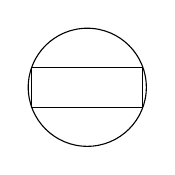
\begin{tikzpicture}[scale=.75]
		\draw (0,0) circle (1); 
		\draw (20:1) -- (160:1) -- (200:1) -- (340:1) -- cycle;
	\end{tikzpicture}
	,
	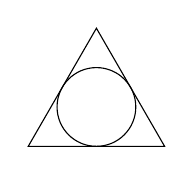
\begin{tikzpicture}
		\draw (0,0) circle (.5);
		\draw (90:1) -- (210:1) -- (330:1) -- cycle;
	\end{tikzpicture}
	\end{sol}
	\end{ex}
	
	\bigskip

	\begin{ex}
	Fill in the missing items in the chart below. (Answer table located in the proof solutions, appendix D)
	
	\begin{tabularx}{.9\textwidth}{@{ } c X c c @{ } }
	\toprule
	sides 	&	name 	& 	diagonals from one vertex	&	total diagonals \\
	\midrule
	3 &&&\\
	4 &&&\\
	7 &&&\\
	&	pentagon && \\
	&	octagon && \\
	&&		9 & \\
	&&		3 & \\
	&&&				27\\
	$n$ &&&\\
	\bottomrule
	\end{tabularx}
	\begin{sol} Answer in Appendix~\ref{sec:proof-answers} \end{sol}
%	\begin{sol}
%	a. triangle, b. 0, c. 0, d. quadrilateral, e. 1, f. 2, g. heptagon, h. 4, i. 14, j. 5, k. 2, l. 5, m. 8, n. 5, o. 20, p. 12, q. dodecagon, r. 54, s. 6, t. hexagon, u. 9, v. 9, w. nonagon, x. 6, y. n-gon, z. $(n-3)$, aa. $\frac{n(n-3)}{2}$
%	\end{sol}
	\begin{prf}

%	\begin{tabular}{@{ } c c p{2.5cm} c @{ } }
	\begin{tabular}{@{ } c c c c @{ } }
	\toprule
	sides 	&	name 	& 	diagonals from one vertex	&	total diagonals \\
	\midrule
	3 & triangle & 0 & 0\\
	4 & quadrilateral & 1 & 2\\
	7 & heptagon & 4 & 14\\
	5 & pentagon & 2 &5\\
	8 & octagon & 5 & 20\\
	12 &	dodecagon &	9 & 54\\
	6 & hexagon		&					3 & 9\\
	9 & nonagon			&	6				&					27\\
	$n$ &n-gon&$(n-3)$& $\frac{n(n-3)}{2}$\\
	\bottomrule
	\end{tabular}
	\end{prf}
	\end{ex}
	
\end{exercises}

%--------------------------------------------------------------------------------------------
			\section{Angle measures}
			\label{sec:regular-polygon-angles}
%--------------------------------------------------------------------------------------------

\subsection{Interior vs.\ exterior angles.}

One of the most surprising conclusions of Euclidean geometry
is that the sum of the angles of any triangle is $180\degree$.

Of course, only 3-sided polygons have an interior angle sum of $180\degree$.
Quadrilaterals, as you know from Section \ref{sec:quad-angle-sum}, 
have an interior angle sum of $360\degree$.

In this section, we seek a formula to find the interior angle sum of any $n$-gon.
We will also review the definition of an \emph{exterior angle}, 
and see an interesting formula for their sum for any $n$-gon.

\subsection{Interior angle measure sum}

The angles labeled in red below constitute the \emph{interior angles} of the hexagon.
Of course, the interior angles generally have different measures, the exception being an equiangular polygon.
	\begin{center}
	\begin{tikzpicture}
		\draw (0,0) coordinate (a)
			-- (2,0) coordinate (b)
			-- (3,1) coordinate (c)
			-- (4,3) coordinate (d)
			-- (1,2.5) coordinate (e)
			-- (-1,1) coordinate (f)
			-- cycle;
		\begin{scope}[red]
		\mangle abf
		\mangle bca
		\mangle [360] cdb
		\mangle dec
		\mangle efd
		\mangle fae
		\end{scope}
	\end{tikzpicture}
	\end{center}
So, how can you determine the interior angle sum? 
The solution, as is frequently the case, is to reduce the problem
to one you already know how to solve: in this case, triangles.

Notice that you can divide any polygons into triangles
by drawing all the diagonals from a single vertex.
	\begin{center}
	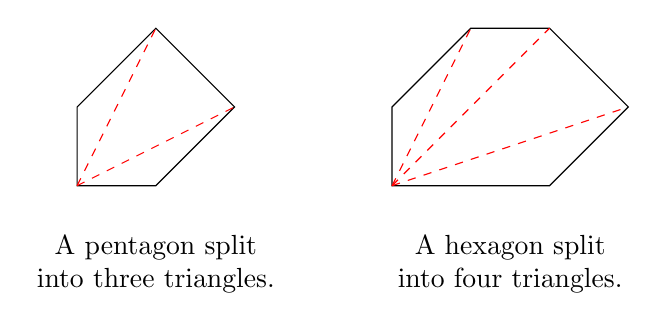
\begin{tikzpicture}
		\draw (0,0) -- (1,0) -- (2,1) -- (1,2) -- (0,1) -- cycle;
		\node [align=center] at (1,-1) {A pentagon split \\ into three triangles.};
		
		\draw (4,0) -- (6,0) -- (7,1) -- (6,2) -- (5,2) -- (4,1) -- cycle;
		\node [align=center] at (5.5,-1) {A hexagon split \\ into four triangles.};
		
		\begin{scope}[red,dashed]
			\draw (0,0) -- (2,1);
			\draw (0,0) -- (1,2);
			\draw (4,0) -- (7,1);
			\draw (4,0) -- (6,2);
			\draw (4,0) -- (5,2);
		\end{scope}
	\end{tikzpicture}
	\end{center}

\noindent \q Do you see the relationship between the number of sides of the polygon and the number of triangles formed by drawing all of the diagonals from one vertex?\\	
	
The key to seeing the answer is that \textit{The angles of each polygon
match up exactly with the angles of the triangles put together!} 
Thus, the angles of a pentagon (which consists of three triangles) sum to 
$3\cdot180\degree=540\degree$.
The angles of a hexagon sum to $4\cdot 180\degree=720\degree$.



\begin{tcolorbox}
\textbf{Sum $S$ of the interior angles of an $n$-gon}\\

\[S=(n-2)180\]

\end{tcolorbox}

\subsection{Exploration:  Exterior angle measure sum}

You may recall, the exterior angles are \emph{not} the angles the rest of the way around the vertex from the interior angles like the ones marked in gray below.  Instead, the exterior angles are angles that form linear pairs with the interior angles, made by extending one side of the polygon at each vertex, like the ones marked red below.
	\begin{center}
	\begin{tikzpicture}[scale=.85]
		\draw (0,0) coordinate (a)
			-- (2,0) coordinate (b)
			-- (3,1) coordinate (c)
			-- (4,3) coordinate (d)
			-- (1,2.5) coordinate (e)
			-- (-1,1) coordinate (f)
			-- cycle;
		\coordinate (b1) at (2,-1); \coordinate (b2) at (3,0);
		\begin{scope}[gray]
			\mangle [360]afb
			\mangle [360]dce
			\mangle [360]edf
			\mangle [360]fea
			\draw (1.75,0) arc (-180:45:.25);
			\draw ($(c)!.25cm!(b)$) arc (-135:63.435:.25);
		\end{scope}
		\node at (1.5,-1) {{\bfseries Not} the exterior angles!};
	\end{tikzpicture}
	\hspace*{1cm}
	\begin{tikzpicture}[scale=.85]
		\draw (0,0) coordinate (a)
			-- (2,0) coordinate (b)
			-- (3,1) coordinate (c)
			-- (4,3) coordinate (d)
			-- (1,2.5) coordinate (e)
			-- (-1,1) coordinate (f)
			-- cycle;
		\draw (b) -- ($(b)!1cm!180:(a)$) coordinate (b1);
		\draw (c) -- ($(c)!1cm!180:(b)$) coordinate (c1);
		\draw (d) -- ($(d)!1cm!180:(c)$) coordinate (d1);
		\draw (e) -- ($(e)!1cm!180:(d)$) coordinate (e1);
		\draw (f) -- ($(f)!1cm!180:(e)$) coordinate (f1);
		\draw (a) -- ($(a)!1cm!180:(f)$) coordinate (a1);
		\begin{scope}[red,thick]
			\mangle a{a1}b
			\mangle b{b1}c
			\mangle c{c1}d
			\mangle [360]d{d1}e
			\mangle e{e1}f
			\mangle f{f1}a
		\end{scope}
		\node at (1.5,-1) {Exterior angles!};
	\end{tikzpicture}
	\end{center}
\noindent \q Draw and mark the exterior angles on the regular octagon below.  Remember:  we only count one exterior angle at each vertex.

	\vspace{0.3cm}
	\begin{center}
	\begin{tikzpicture} [scale=0.9]
		\draw (22.5:2) -- (67.5:2) -- (112.5:2) -- (157.5:2)
			-- (202.5:2) -- (247.5:2) -- (292.5:2) -- (337.5:2) -- cycle;
	\end{tikzpicture}
	\end{center}
	
	\vspace{0.1cm}

\begin{enumerate}
\item  Calculate the sum of the interior angles of the octagon above.
\item  Calculate the individual interior angle measure and write them in the octagon.
\item  Calculate and write in the measures of the exterior angles.
\item  Calculate the sum of the exterior angles.
\end{enumerate}

\noindent \q What is the sum of the exterior angles of a square?  Do you know the sum of the exterior angles of a 20-gon?\\
	
	
To justify the sum of the exterior angles of a polygon, you need to take advantage of the fact that exterior angles form linear pairs with interior angles. Therefore, if you sum all the linear pairs and subtract the interior angles, what remains are the exterior angles.
\[ 
\begin{array}{r @{ = } c @{ - } c c l}
\text{Exterior angle sum } & \text{ linear pairs } & \text{ interior angles } \\
& [n\cdot (180)] & [(n-2) \cdot 180] \\
& [180n]& [180n-360] \\
&180n&180n+360&=&\fbox{360}\\
\end{array}
\]

\begin{tcolorbox}
\textbf{Sum of the Exerior angles of an $n$-gon}\\

\begin{center}
\dots is always $360\degree$
\end{center}

\end{tcolorbox}

\noindent \q For a dodecagon, find the sum of the interior angles and the sum of the exterior angles.

\paragraph{Answer} A dodecagon has 12 sides (that is, $n=12$),
so the interior angle sum is $(12-2)\cdot 180 = 1800\degree$,
and the exterior angle sum is $360\degree$.

\subsection{Application to regular polygons}

Recall that a regular polygon is equiangular. 
The formulas in the previous section apply to all polygons,
but if a polygon is regular, 
then you have the additional information that all angles are congruent.
Not only do you know the angle sum,
but you can also find what each measure is.

\noindent \q Find each interior and exterior angle of a regular 20-gon.

\paragraph{Answer} The sum of the interior angles is $(20-2)180=3240$,
and since the polygon is regular, the $3240\degree$ is divided evenly by the
twenty angles, making each one $\frac{3240}{20}=162\degree$

The sum of the exterior angles is 360, and since the polygon is regular,
each exterior angle must measure $\frac{360}{20}=18\degree$.

\noindent \q As a final thought, what do you notice about the two answers to the previous example problem?  If you found the individual exterior angle first, what would be an easy way to find the individual interior angle?\footnote{Hint:  For more efficient and easier problem solving, always use the exterior angles in regular polygons!}

\vfill

\begin{exercises}

	\begin{ex} \e Make note cards for:  \textbf{Interior/Exterior Angles}, \textbf{Sum of Interior Angles}, \textbf{Sum of Exterior Angles}
	\begin{sol}
	Note cards
	\end{sol}
	\end{ex}
	
	\begin{ex}
	\e Find the sum of the interior angles for each polygon below:\\
	\begin{tabular}{p{4cm} p{4cm} p{4cm} }
	(a) pentagon & (b) octagon & (c) 96-gon \\\\\\
	(d) quadrilateral & (e) heptagon & (f) decagon \\\\\\
	\end{tabular}
	
	\begin{sol}
	(a) $540\degree$, (b) $1080\degree$, (c) $16920\degree$,
	(d) $360\degree$, (e) $900\degree$, (f) $1440\degree$
	\end{sol}
	\end{ex}

	\begin{ex}
	\e Find the sum of the exterior angles for each polygon below:\\
	\begin{tabular}{p{4cm} p{4cm} p{4cm} }
	(a) hexagon & (b) triangle & (c) 17-gon \\\\\\
	\end{tabular}
	
	\begin{sol}
	(a) $360\degree$, (b) $360\degree$, (c) $360\degree$,
	\end{sol}
	\end{ex}

	\begin{ex}
	\e Solve for $x$ in the diagram below.
	\begin{center}
	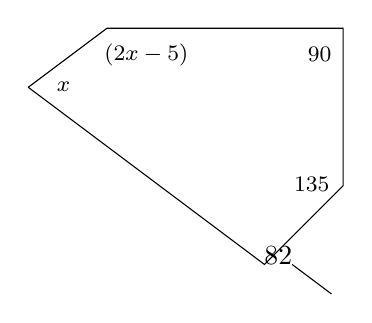
\begin{tikzpicture}[font=\footnotesize]
		\draw (-3,2.25) coordinate (a) -- (0,0) node [above right,pos=0.08] {$x\degree$} coordinate (b) 
			-- (1,1) coordinate [label={[shift={(-.4,-.2)}]135\degree}] (c)
			-- (1,3) coordinate [label={[shift={(-.3,-.55)}]90\degree}] (d) 
			-- (-2,3) coordinate [label={[shift={(.5,-.6)}]$(2x-5)\degree$}](e) 
			-- (-3,2.25) coordinate (f);
		\labelang [0.5]bca{$82\degree$}
%		\labelang [.4] fae{$x\degree$}
	\draw (b)-- (0.5,-0.375);
	\end{tikzpicture}
	\end{center}
	\begin{sol}
	74
	\end{sol}
	\end{ex}
	
	\newpage
	
	\begin{ex}
	\e Find the measure of one exterior angle for each polygon below:
	
	\begin{tabular}{p{3.5cm} p{4cm} p{3.5cm} }
	(a) regular hexagon & (b) regular dodecagon & (c) regular octagon \\\\\\
	(d) regular pentagon & (e) regular nonagon & (f) regular decagon \\\\\\
	\end{tabular}
	\begin{sol}
	(a) $60\degree$, (b) $30\degree$, (c) $45\degree$,
	(d) $72\degree$, (e) $40\degree$, (f) $36\degree$	
	\end{sol}
	\end{ex}
	
	\begin{ex}
	\e Find the measure of one interior angle for each polygon below:
	
	\begin{tabular}{p{3.5cm} p{4cm} p{3.5cm} }
	(a) regular hexagon & (b) regular dodecagon & (c) regular octagon \\\\\\
	(d) regular pentagon & (e) regular nonagon & (f) regular decagon \\\\\\
	\end{tabular}
	\begin{sol}
	(a) $120\degree$, (b) $150\degree$, (c) $135\degree$,
	(d) $108\degree$, (e) $140\degree$, (f) $144\degree$	
	\end{sol}
	\end{ex}

	\begin{ex}
	\e The interior angles of a certain polygon sum to $1260\degree$. 
	Name the polygon.
	\begin{sol}
	nonagon
	\end{sol}
	\end{ex}
	
	\medskip

	\begin{ex}
	\e Each exterior angle of a regular polygon is $18\degree$.
	How many sides does the polygon have?
	\begin{sol}
	20
	\end{sol}
	\end{ex}
	
	\medskip

	\begin{ex}
	\e Each interior angle of a regular polygon is $175\degree$.
	How many sides does the polygon have?
	\begin{sol}
	72
	\end{sol}
	\end{ex}
	
	\medskip

\end{exercises}

%--------------------------------------------------------------------------------------------
			\section{Regular Polygons}
%--------------------------------------------------------------------------------------------

As you may remember,
there are many different formulas to find the areas of different figures.
Polygons can be quite complicated, so if you want to find its area,
you typically have to break it down in to simpler polygons.
There is, however, one formula that is useful for finding the area
of any \emph{regular polygon}.

\subsection{Terminology}

As we found out earlier in the chapter, every regular polygon can be inscribed
in a circle.  (Or, in other words, you can always circumscribe a circle about
any regular polygon.)  As we saw with squares and equilateral triangles, it is the convention to use $s$ for the side length. 
	\begin{center}
	\begin{tikzpicture}
		\draw [thick] (90:2) -- (162:2) node [above, pos=0.5] {$s$} -- (234:2) -- (306:2) -- (18:2) -- (90:2);
		\draw [gray] (0,0) coordinate (o) circle (2);
		\draw (0,0)-- (162:2) node [below, pos=0.2] {$\theta$};
		\draw (0,0)-- (234:2);
		\draw (0,0)-- (306:2);
		\draw (0,0)-- (18:2);
		\draw (0,0)-- (90:2);
		\draw [dashed] (0,0)-- ($(234:2)!.5!(306:2)$) coordinate (d) node [pos=0.5,right] {$\frac{\theta}{2}$};
		\fillpoints {o}
		\perpbox d{306:2}o
	\end{tikzpicture}
	\hspace*{2cm}
	\begin{tikzpicture}
		\draw [thick] (22.5:2) coordinate (r) -- (67.5:2) -- (112.5:2) -- (157.5:2)
			-- (202.5:2) -- (247.5:2) coordinate (a) 
			-- (292.5:2) coordinate (b) -- (337.5:2) -- cycle;
		\coordinate [label=left:\pnt C] (o) at (0,0);
		\draw [gray] (o) circle (2);
		\draw (o) -- ($(a)!.5!(b)$) coordinate (d)  node [midway,left] {$a$};
		\draw (o) -- (r) node [midway,above] {$r$};
		\fillpoints {o}
		\perpbox dbo
	\end{tikzpicture}
	\end{center}
When you do so, 
it makes sense to define the following:
\begin{description}
\item[center] The center ($C$) of a regular polygon is the center of its circumscribed circle.
\item[radius] The radius ($r$) of a regular polygon is the radius of its circumscribed circle.
\item[apothem] The apothem ($a$) of a regular polygon is a segment from
the center of a polygon perpendicular to a side of the polygon. 
The apothem always bisects a side of the polygon. \q Why?
\medskip
\item[central angle] The central angle ($\theta$) of a regular polygon is the angle formed by two radii with its vertex on the center of the polygon.  The measure of the central angle of an $n$-gon is $\frac{360}{n}$. \q Why?
\end{description}

\medskip
\medskip

It is unusual to think of a regular polygon as having a center, a radius and a central angle---those are terms that we usually associate uniquely with circles---but regular polygons have them too!\\

Before finding the area of a regular polygon, one thing to notice is that you can form a right triangle with the apothem, radius, and half a side $s$.
Also, using the fact that central angles are congruent and that there are $n$ of them in an $n$-gon, it is also possible to fill in one of the angles of the triangle.  The polygon below is a decagon ($n=10$).
	\begin{center}
	\begin{tikzpicture}
		%\draw [help lines] (0,-2) grid (10,4);
		\coordinate (o) at (0,0);
		\draw (0:2) -- (36:2) -- (72:2) -- (108:2) 
			-- (144:2) -- (180:2) -- (216:2) -- (252:2) coordinate (s1)
			-- (288:2) coordinate (s2) -- (324:2) -- cycle;
		\draw (o) -- ($(s1)!.5!(s2)$) coordinate (a) node[midway,left] {$a$};
		\draw (o) -- (s2) node [midway,right] {$r$};
		\node [below] at ($(a)!.5!(s2)$) {$\frac{s}{2}$};
		\draw [gray] (o) circle (2);
		\perpbox a{s2}o
		\fillpoints{o}
		\node [right,align=left] at (180:7) 
			{$\begin{array}{rcl} 
				\theta~=~\dfrac{360\degree}{10}&=&36\degree \\[3ex] 
				\dfrac{\theta}{2}~=~\dfrac{36\degree}{2}&=&18\degree \end{array}$};
		\draw [->] (-3.1,-0.8) to [bend right] (279:0.4);		
%		\draw [->] (6.6,-1.4) to [bend left] (285:1.9);
	\end{tikzpicture}
	\end{center}
So, you can draw a right triangle and find one of the angles. 
Get ready for \hyperref[sec:SohCahToa]{right triangle trigonometry}!

\noindent \q Find the apothem of a regular octagon with radius $3~cm$.

\bigskip

\subsection{Area of a regular polygon}

Let's review.\\  
\noindent \q How many sides does an $n$-gon have?\\  
\noindent \q How many radii does an $n$-gon have?\\  
\noindent \q How many apothems does an $n$-gon have?\\  
\noindent \q How many central angles does an $n$-gon have?\\  
\noindent \q How many congruent isosceles triangles are formed when all of the radii are drawn in an $n$-gon?

\newpage

The formula for the area of a regular polygon can be derived by summing the areas of all the congruent isosceles triangles.

There are $n$ isosceles triangles\footnote{Each isosceles triangle is split into two congruent right triangles comprised of the radius, apothem and half of a side of the polygon}, all of which have area $\frac{1}{2}\cdot s \cdot a$.

\[ A = (n)\left (\frac{1}{2}\cdot s \cdot a\right ) = \frac{1}{2} a \cdot ns\]

Recognize that $ns$ is the number of sides times the side length, that is, the perimeter ($p$), and you have derived a formula for the area.

\begin{tcolorbox}
\textbf{Area $A$ of any regular $n$-gon with perimeter $p$}\\

\[A=\frac{1}{2}ap\]

\end{tcolorbox}


\paragraph{Example} Find the area of a regular pentagon with side length 10\, m.

\paragraph{Answer} You need the apothem and the perimeter. 
The perimeter is easy here: it's $50~m$. 
The apothem can be found with a quick sketch, an angle calculation,
and some right triangle trig:
	\begin{center}
	\begin{tikzpicture}
		%\draw [help lines] (-5,-2) grid (5,4);
		\coordinate (o) at (0,0);
		\draw [gray] (18:2) -- (90:2) -- (162:2) 
			-- (234:2) coordinate (s1) -- (306:2) coordinate (s2)
			-- cycle;
		\draw (o) -- ($(s1)!.5!(s2)$) coordinate (a) node[midway,right] (ap) {$a$};
		\draw (s1) -- (a);
		\draw (o) -- (s1);
		\node [below] at ($(s1)!.5!(a)$) {$5\, \text{m}$};
		%\draw [gray] (o) circle (2);
		\perpbox ao{s1}
		\fillpoints{o}
		\node [below right,align=left] at (-5.5,1) 
			{$\begin{array}{rcl} 
				\dfrac{360\degree}{5}&=&72\degree \\[2ex] 
				\dfrac{72\degree}{2}&=&36\degree \end{array}$};
		\node [below right, align = left]at (2.25,2) 
			{$\begin{array}{rcl} 
				\tan (36\degree) &=& \dfrac{5}{a} \\[2ex]
				 a &=& \dfrac{5}{\tan (36\degree)}\\[2ex]
				 a &=& 6.882
				\end{array}
			$};
		\draw [->] (-2.8,-.8) to [bend right] (-0.1,-0.3);
		\draw [->] (3.6,-.7) to [bend left] (ap);
	\end{tikzpicture}
	\end{center}
So the area is $A=\frac{1}{2}(6.882~m)(50~m)\approx 172.048~m^2$.

\begin{exercises}

	\begin{ex} \e Make note cards for:  \textbf{Regular Polygon (include center, radius, apothem and central angle)} and \textbf{Area of a Regular Polygon}.
	\begin{sol}
	Note cards
	\end{sol}
	\end{ex}
	
	\begin{ex} \e Find the area of a regular pentagon with an apothem of length 7 inches.
	
\begin{flushright}
\begin{tikzpicture}

	\coordinate [label=above right:] (X) at (0,0);

	\draw 	(18:2) --
			(90:2) node [above, pos = 1] {} --
			(162:2) node [above, pos = 1] {}--
			(234:2) --
			(306:2) --
			(18:2);
	
	\draw 	[dashed] (0,0) -- (0,-1.618) node [right, pos = 0.5] {$7$ in};
	\perpbox {0,-1.618}{306:2}X
	
	\foreach \point in {X} \fill (\point) circle (1.5pt);	

\end{tikzpicture}	
\end{flushright}

	\begin{sol}
	178 $in^2$
	\end{sol}
	\end{ex}
	
	\smallskip
	
	\begin{ex}
	\e Find the area of a regular dodecagon with radius of length 16 meters.
	
\begin{flushright}
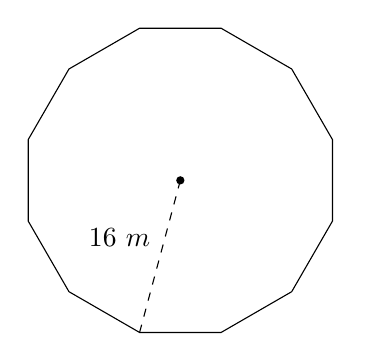
\begin{tikzpicture}

	\coordinate [label=above right:] (X) at (0,0);

	\draw 	(315:2) --
			(345:2) node [above, pos = 1] {} --
			(15:2) node [above, pos = 1] {}--
			(45:2) --
			(75:2) --
			(105:2) --
			(135:2) --
			(165:2) --
			(195:2) --
			(225:2) --
			(255:2) --
			(285:2) --
			(315:2);
	
	\draw 	[dashed] (0,0) -- (255:2) node [above left, pos = 0.5] {$16~m$};
	
	\foreach \point in {X} \fill (\point) circle (1.5pt);	

\end{tikzpicture}	
\end{flushright}
	
	\begin{sol}
	768 $m^2$
	\end{sol}
	\end{ex}
	
	\smallskip
	
	\begin{ex}
	\e Find the area of a regular octagon with apothem of length 30 feet.
	\begin{sol}
	2982.338 $ft^2$
	\end{sol}
	\end{ex}
	
	\bigskip

	\begin{ex}
	\e Find the area of a regular heptagon with a perimeter of 70 centimeters.
	\begin{sol}
	363.391 $cm^2$
	\end{sol}
	\end{ex}

	\bigskip
	
	\begin{ex} If a regular 15-gon is inscribed in a circle, how many degrees of arc are there between vertices?
	 
	\begin{sol}
	24\degree, same as the central angle measure
	\end{sol}
	\end{ex}
	
	\medskip
	
	\begin{ex} \e The two diagrams below each consist of a circle  with a radius of 10.  The diagram on the left has an equilateral triangle inscribed in the circle and an equilateral triangle circumscribed about the circle.  The diagram on the right has a square inscribed in the circle and a square circumscribed about the circle.  For each figure:
	\begin{exparts}
	\item Give the area of the circumscribed polygon.
	\item Give the area of the inscribed polygon.
	\item Give the ratio between the areas (larger to smaller).
	\end{exparts}
	
	\begin{center}
	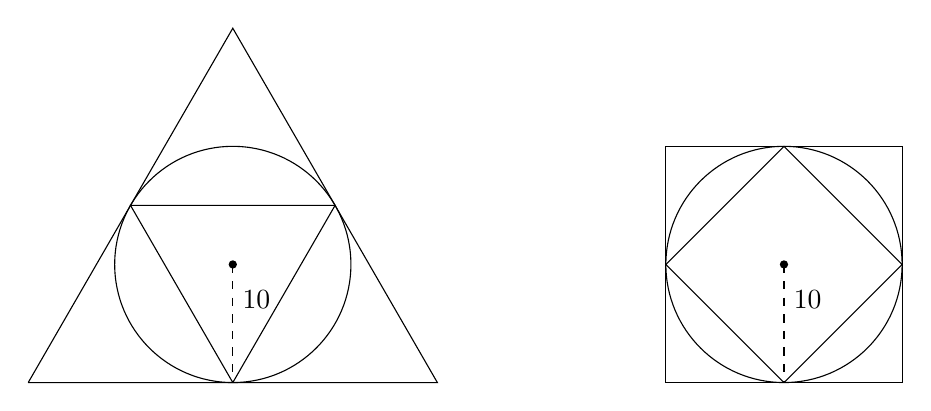
\begin{tikzpicture}

	\coordinate [label=above right:] (X) at (0,0);
	\coordinate (A) at (270:1.5);
	\coordinate (B) at (30:1.5);
	\coordinate (C) at (150:1.5);
	\coordinate (D) at (210:3);
	\coordinate (E) at (330:3);
	\coordinate (F) at (90:3);
	
	\draw (X) circle (1.5cm);
	\draw 	(A)--(B)--(C)--(A);
	\draw 	(D)--(E)--(F)--(D);
	
	\draw 	[dashed] (0,0) -- (270:1.5) node [right, pos = 0.3] {10};
	
	\foreach \point in {X} \fill (\point) circle (1.5pt);	
	
	\begin{scope} [xshift=7cm]
	\coordinate [label=above right:] (Y) at (0,0);
	\coordinate (M) at (270:1.5);
	\coordinate (N) at (0:1.5);
	\coordinate (O) at (90:1.5);
	\coordinate (P) at (180:1.5);
	\coordinate (Q) at (-1.5,-1.5);
	\coordinate (R) at (1.5,-1.5);
	\coordinate (S) at (1.5,1.5);
	\coordinate (T) at (-1.5,1.5);
	
	\draw (Y) circle (1.5cm);
	\draw 	(M)--(N)--(O)--(P)--(M);
	\draw 	(Q)--(R)--(S)--(T)--(Q);
	
	\draw 	[dashed] (0,0) -- (270:1.5) node [right, pos = 0.3] {10};
	
	\foreach \point in {Y} \fill (\point) circle (1.5pt);
	\end{scope}

\end{tikzpicture}
\end{center}	

	\begin{sol}
	Triangle:\\
	\begin{exparts}
	\item $300\sqrt{3}$
	\item $75\sqrt{3}$
	\item 4:1 or $\frac{4}{1}$
	\end{exparts}
	Square:\\
	\begin{exparts}
	\item 400
	\item 200
	\item 2:1 or $\frac{2}{1}$
	\end{exparts}
	
	\end{sol}
	\end{ex}
	
	\bigskip
	
	\begin{ex} \e In the previous problem, the radius of the circle is what part of the polygon inscribed in the circle?  The radius of the circle is what part of the polygon circumscribed about the circle?
	
	\begin{sol}
	The radius of the circle is the radius of the polygon inscribed in the circle and the apothem of the polygon circumscribed about the circle.
	\end{sol}
	\end{ex}
	
	\medskip
	
	\begin{ex} \e If a regular polygon has exterior angles of $1^\circ$, how many sides does it have?  If you were to try and draw this, what would it look like?
	 
	\begin{sol}
	360 sides, it would probably look like a circle.
	\end{sol}
	\end{ex}
	
	\medskip
	
	
\end{exercises}

%--------------------------------------------------------------------------------------------
			\section{Exploration:  Is a Circle a Polygon?}
%--------------------------------------------------------------------------------------------

Is a circle a polygon with an infinite number of sides that are infinitely small?  Let's explore this ``point of view.'' Question 11.3.7 had you calculate the areas of inscribed and circumscribed polygons relative to a \textbf{circle with the same radius of 10}.  Then you were asked to create a ratio between the circumscribed area and the inscribed area.  Considering what you found out in question 11.3.7 and what is pictured below, what do you think will happen to the ratio of areas as the number of sides increases for polygons inscribed in and circumscribed about a circle of radius 10?  Do you think the ratio can be one?  If it is, what does that mean?  The first two rows are filled in with the answers to question 11.3.7.  You may make the calculations necessary for this exploration by calculator or by using a spreadsheet (spreadsheet is recommended).

\begin{center}
	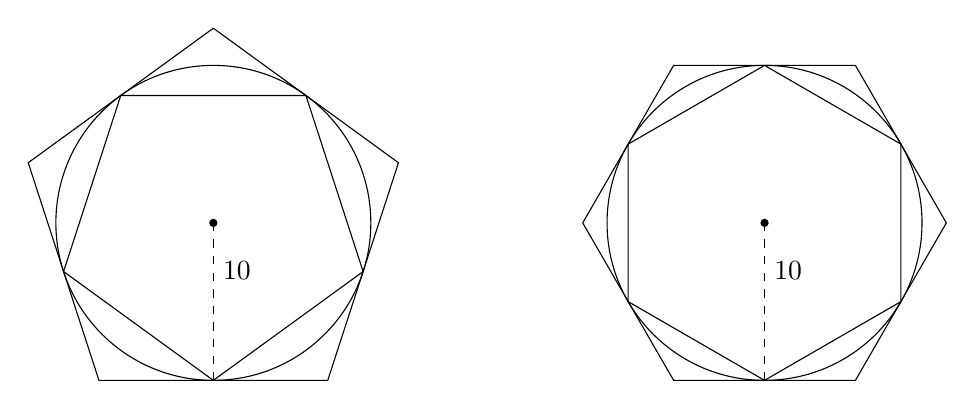
\begin{tikzpicture}

	\coordinate [label=above right:] (X) at (0,0);
	\coordinate (A) at (270:2);
	\coordinate (B) at (342:2);
	\coordinate (C) at (54:2);
	\coordinate (D) at (126:2);
	\coordinate (E) at (198:2);
	\coordinate (F) at (234:2.472);
	\coordinate (G) at (306:2.472);
	\coordinate (H) at (18:2.472);
	\coordinate (I) at (90:2.472);
	\coordinate (J) at (162:2.472);
	
	\draw (X) circle (2cm);
	\draw 	(A)--(B)--(C)--(D)--(E)--(A);
	\draw 	(F)--(G)--(H)--(I)--(J)--(F);
	
	\draw 	[dashed] (0,0) -- (270:2) node [right, pos = 0.3] {10};
	
	\foreach \point in {X} \fill (\point) circle (1.5pt);	
	
	\begin{scope} [xshift=7cm]
	\coordinate [label=above right:] (Y) at (0,0);
	\coordinate (K) at (270:2);
	\coordinate (L) at (330:2);
	\coordinate (M) at (30:2);
	\coordinate (N) at (90:2);
	\coordinate (O) at (150:2);
	\coordinate (P) at (210:2);
	\coordinate (Q) at (300:2.309);
	\coordinate (R) at (0:2.309);
	\coordinate (S) at (60:2.309);
	\coordinate (T) at (120:2.309);
	\coordinate (U) at (180:2.309);
	\coordinate (V) at (240:2.309);
	
	\draw (Y) circle (2cm);
	\draw 	(K)--(L)--(M)--(N)--(O)--(P)--(K);
	\draw 	(Q)--(R)--(S)--(T)--(U)--(V)--(Q);
	
	\draw 	[dashed] (0,0) -- (270:2) node [right, pos = 0.3] {10};
	
	\foreach \point in {Y} \fill (\point) circle (1.5pt);
	\end{scope}

\end{tikzpicture}
\end{center}	

\newpage

In the table below, \textbf{n} is the number of sides of the polygon, \textbf{$\frac{\theta}{2}$} is half of the central angle measure, \textbf{a} is the apothem, \textbf{s} is the side length, \textbf{p} is the perimeter, \textbf{Area} is the area of the inner or outer polygon and \textbf{Ratio} is the ratio of circumscribed to inscribed polygon areas $\left(\dfrac{circumscribed}{inscribed} \right)$.  Round your ratio to 4 or more decimal places.


	\hfill \textbf{Circumscribed Polygon} \hspace{1cm} \textbf{Inscribed Polygon} \hspace*{1.5cm}\\
\begingroup	
\renewcommand*{\arraystretch}{2}	
\begin{tabular}{| c | @{\hspace{0.2cm}} c @{\hspace{0.2cm}}|  
			@{\hspace{0.2cm}}c @{\hspace{0.2cm}} | @{\hspace{0.2cm}} c @{\hspace{0.2cm}}| @{\hspace{0.2cm}} c @{\hspace{0.2cm}}| @{\hspace{0.2cm}} c @{\hspace{0.2cm}}|  
			@{\hspace{0.2cm}}c @{\hspace{0.2cm}} | @{\hspace{0.2cm}} c @{\hspace{0.2cm}}| @{\hspace{0.2cm}} c @{\hspace{0.2cm}}|@{\hspace{0.2cm}} c @{\hspace{0.2cm}}| @{\hspace{0.2cm}} c @{\hspace{0.2cm}}|} \hline
	\toprule
	n &	$\frac{\theta}{2}$ & a & s & p & Area & a & s & p & Area & Ratio\\ \hline
	
	3 & 60 & 10 & 34.64 & 103.92 &519.61&5.00&17.32&51.96&129.90&4.0000\\ \hline
	
	4 & 45 & 10 & 20&80&400&7.07&14.14&56.57&200&2.0000\\ \hline
	
	5 & 36 &&&&&&&&&\\ \hline
	
	6 & 30 &&&&&&&&&\\ \hline
	
	8 &  &&&&&&&&&\\ \hline
	
	10 &&&&&&&&&&\\ \hline
	
	12 &&&&&&&&&&\\ \hline
	
	20 &&&&&&&&&&\\ \hline
	
	36 &&&&&&&&&&\\ \hline
	
	90 &&&&&&&&&&\\ \hline
	
	180 &&&&&&&&&&\\ \hline
	
	360 &&&&&&&&&&\\ \hline
	
	720 &&&&&&&&&&\\ \hline
	
	1440 &&&&&&&&&&\\ \hline
	
	2880 &&&&&&&&&&\\
	\bottomrule
	\end{tabular}
\endgroup	


\begin{exercises}

	\begin{ex} \e For what value of n (\# of sides) did the ratio reach 1.00?
	 
	\begin{sol}
	n = 90
	\end{sol}
	\end{ex}
	
	\smallskip
	
	\begin{ex} \e For what value of n (\# of sides) did the ratio reach 1.000?
	 
	\begin{sol}
	n = 180
	\end{sol}
	\end{ex}
	
	\smallskip
	
	\begin{ex} \e For your largest value of n, what was the difference between the circumscribed and inscribed areas?  Give the average of the two areas to three decimal places.
	 
	\begin{sol}
	n=2880, difference = 0.000374, avg. area = 314.159
	\end{sol}
	\end{ex}
	
	\smallskip
	
	\begin{ex} \e Give the area of a circle with radius of 10.
	 
	\begin{sol}
	314.159
	\end{sol}
	\end{ex}
	
	\smallskip
	
	\begin{ex} Find the area of a regular polygon with individual interior angle measures of $140^\circ$ and a side length of 5 cm.
	 
	\begin{sol}
	$154.55~cm^2$
	\end{sol}
	\end{ex}
	
	\vfill
	
	\begin{ex} A regular 20-gon is inscribed in a circle with an area of 225$\pi$ square meters.  What is the perimeter of the polygon.
	 
	\begin{sol}
	$93.86~m$
	\end{sol}
	\end{ex}
	
	\vfill
	\newpage
	
	\begin{ex} \e Consider the following diagram with a regular octagon inscribed in a circle.  Solve for $s$ and $t$. (Hint:  think inscribed angles)

\newdimen\R
\R=2.0cm

\begin{center}
\begin{tikzpicture} [scale=0.8]
    % Indicate the boundary of the regular polygons
    \draw  circle (\R) ;
    \draw(0:\R) \foreach \x in {45,90,...,359} {
            -- (\x:\R)
        } -- cycle (90:\R);
        
    \draw (2,0)--(135:2);   
    
    \coordinate [label=below left:$s^\circ$] (s) at (1.9,0.1);
	\coordinate [label=above right:$t^\circ$] (t) at (-0.9,1.1); 

\end{tikzpicture}
\end{center}
	 
	\begin{sol}
	$t=45$, $s=90$
	\end{sol}
	\end{ex}
	
	\medskip
	
	\begin{ex}
	Consider a circle of radius 12 meters inscribed in a regular hexagon.  Find the \textbf{exact} area of the shaded region.

\begin{flushright}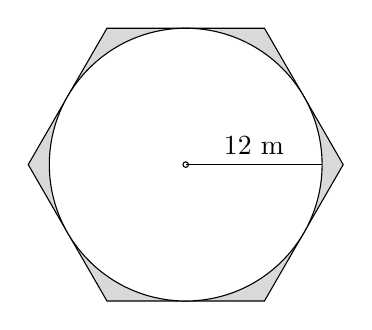
\begin{tikzpicture}
	\filldraw [fill=gray!30,draw=black](0:2)--(60:2)--(120:2)--(180:2)--(240:2)--(300:2)--cycle;
	\filldraw [fill=white,draw=black] (0,0) circle ({sqrt(3)});
	\draw (0,0)--({sqrt(3)},0) node [above, pos=0.5] {12 m};
	\draw (0,0) circle (1pt);
\end{tikzpicture}\end{flushright}
	\begin{sol}
	($288 \sqrt{3} - 144 \pi$) $m^2$
	\end{sol}
	\end{ex}
	
	\medskip
	
	\begin{ex}  \textbf{Challenge:  }  Construct a square inscribed in the circle below.\\
	\begin{center}
	\begin{tikzpicture}
	\draw (0,0) circle (2cm);
	\fill (0,0) circle (1.5pt);
	\end{tikzpicture}
	\end{center}
	\begin{sol}
	Construction
	\end{sol}
	\end{ex}
	
	\newpage
	
	\begin{ex} \textbf{Challenge:  }On the axes below, plot points \textbf{A} $(-2,0)$ and \textbf{B} $(2,0)$.  
	
	
	\begin{exparts}
	\item Label the points of a regular pentagon with side $\overline{AB}$.  

			\begin{flushright}
			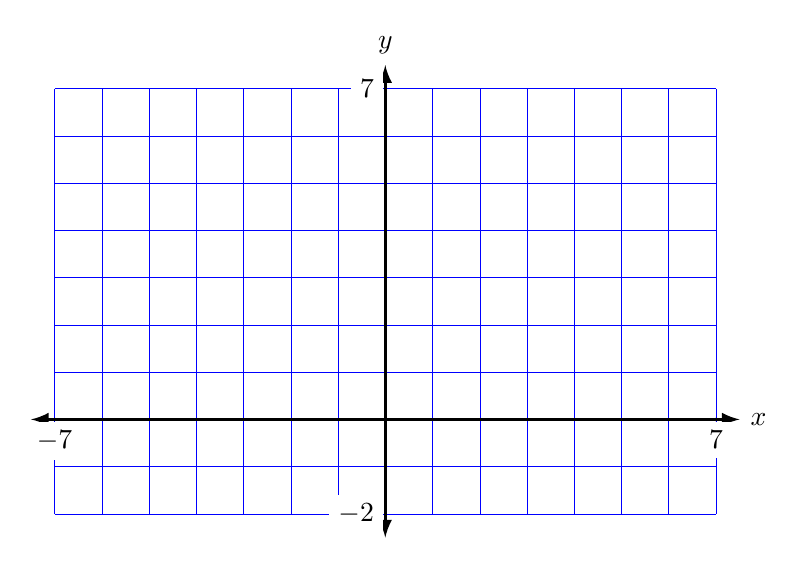
\begin{tikzpicture}[scale=.6]
				\draw [help lines,blue] (-7,-2) grid (7,7);
				\draw [very thick,latex-latex] (-7.5,0)--(7.5,0) node [right] {$x$};
				\draw [very thick,latex-latex] (0,-2.5)--(0,7.5) node [above] {$y$};	
				\foreach \x in {-7,7} 
					\draw (\x cm,1pt) -- (\x,-1pt)	node[anchor=north,fill=white]{$\x$};
				\foreach \y in {-2,7} 
					\draw (1pt, \y cm) -- (-1 pt, \y cm) node[anchor=east,fill=white] {$\y$};			
			\end{tikzpicture}
			\end{flushright}

\vfill
						
	
	\item Sketch a regular pentagon inscribed at the midpoints of each side of the pentagon.  What is the similarity ratio of inner to outer pentagons.
	\vfill
	\item What is the equation of the circle that circumscribes the original pentagon.
	\vfill
	\end{exparts}	
	
	\begin{sol}
	\begin{exparts}
	\item $C$ $(3.24,3.80)$, $D$ $(0,6.15)$, $E$ $(-3.24,3.80)$
	\item 0.81:1 or $\frac{81}{100}$
	\item $x^2 + (y - 2.75)^2 = (3.4)^2$
	\end{exparts}
	\end{sol}
	\end{ex}
	
	\newpage
	
	\begin{ex}  \textbf{Challenge:  }  Construct an equilateral triangle inscribed in the circle below.  Be sure to consider the measure of central angles and arcs between the vertices.\\
	\begin{center}
	\begin{tikzpicture}
	\draw (0,0) circle (2cm);
	\fill (0,0) circle (1.5pt);
	\end{tikzpicture}
	\end{center}
	\begin{sol}
	Construction
	\end{sol}
	\end{ex}
	
\end{exercises}	

%--------------------------------------------------------------------------------------------
			\section{Mixed Review}
%--------------------------------------------------------------------------------------------

\noindent \textbf{Drawings are not necessarily drawn to scale.  Answers should be simplified and may be left as exact answers or rounded to two (2) decimal places, unless otherwise specified.}

\begin{exercises}

	\begin{ex} \e If an exterior angle of a regular polygon has a measure of $30^\circ$, name the polygon.
	
	\begin{sol}
	Dodecagon
	\end{sol}
	\end{ex}
	
	\medskip
	
	\begin{ex} \e If an interior angle of a regular polygon has a measure of $144^\circ$, name the polygon.
	
	\begin{sol}
	Decagon
	\end{sol}
	\end{ex}
	
	\medskip
	
	\begin{ex}  What is the measure of an interior angle of a regular 30-gon.  How many diagonals can be drawn in a 30-gon.
	
	\begin{sol}
	$168\degree$, 405 diagonals
	\end{sol}
	\end{ex}
	
	\medskip
	
	\begin{ex} \e If a regular polygon has interior angles of $177^\circ$, how many sides does it have?
	
	\begin{sol}
	120 sides
	\end{sol}
	\end{ex}
	
	\medskip
	
	\begin{ex}  If a regular hexagon has side length of 4 inches, what is the circumference of the circle that circumscribes it?
	
	\begin{sol}
	$8\pi~in$
	\end{sol}
	\end{ex}
	
	\medskip
		
	\begin{ex} \e Find the area of a regular octagon with a radius of length 8 cm.

\begin{flushright}
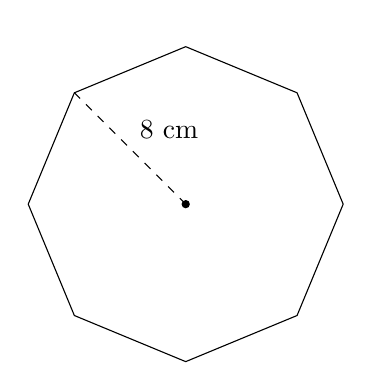
\begin{tikzpicture}

	\coordinate [label=above right:] (X) at (0,0);

	\draw 	(0:2) --
			(45:2) --
			(90:2) node [above, pos = 1] {} --
			(135:2) node [above, pos = 1] {}--
			(180:2) --
			(225:2) --
			(270:2) --
			(315:2) --
			(0:2);
	
	\draw 	[dashed] (0,0) -- (135:2) node [above right, pos = 0.5] {$8$ cm};
	
	\foreach \point in {X} \fill (\point) circle (1.5pt);	

\end{tikzpicture}	
\end{flushright}
	
	\begin{sol}
	$181.02~cm^2$
	\end{sol}
	\end{ex}
	
	\medskip
	
	\begin{ex}  A regular decagon is inscribed in a circle.  The decagon has an apothem of length 4 meters.  What is the area of the circle?
	
	\begin{sol}
	$55.57~m^2$
	\end{sol}
	\end{ex}
	
	\newpage
	
	\begin{ex}  \textbf{Challenge: } Consider the regular hexagon below.  Find the \textbf{exact} area of the shaded region.

\begin{flushright}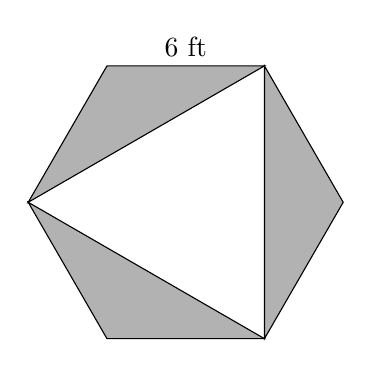
\begin{tikzpicture}

	\filldraw[fill=black!30,draw=black] (60:2)--(-60:2)--(0:2)--cycle;
	\filldraw[fill=black!30,draw=black] (60:2)--(180:2)--(120:2)--cycle;
	\filldraw[fill=black!30,draw=black] (180:2)--(300:2)--(240:2)--cycle;
	
	\node [above] at (0,{sqrt(3)}) {6 ft};

\end{tikzpicture}\end{flushright}
	
	\begin{sol}
	$27\sqrt{3}~ft^2$
	\end{sol}
	\end{ex}
	
	\medskip
	
	\begin{ex}  \textbf{Challenge: } If the area of a regular hexagon is $\frac{147\sqrt{3}}{2}$ square feet, what is the length of one of its sides?
	
	\begin{sol}
	$7~ft$
	\end{sol}
	\end{ex}
	
	\bigskip
	
	\begin{ex}  \textbf{Challenge:  }Using a compass and straightedge, construct a regular hexagon with the given side length below.  Hint:  You may want to construct this hexagon inside a circle.\\\\

\begin{center}

\begin{tikzpicture}

	\draw (0,0)-- node [below,midway] {$side$} (3,0);

\end{tikzpicture}
\end{center}

\vfill
	
	\begin{sol}
	Construction
	\end{sol}
	\end{ex}
	
\end{exercises}	